\documentclass[runningheads]{res/templates/llncs}
%
\usepackage{graphicx}
\usepackage[utf8]{inputenc}
\usepackage[hyphens]{url}
\usepackage{hyperref}
\usepackage{draftwatermark}

\SetWatermarkText{Preprint – to be published in ICCHP 2020}
\SetWatermarkColor[gray]{0.5}
\SetWatermarkFontSize{1cm}
\SetWatermarkAngle{90}
\SetWatermarkHorCenter{2cm}

\begin{document}

\title{An Audio-Based 3D Spatial Guidance AR System for Blind Users}

\titlerunning{Audio-Based 3D Spatial Guidance}

\author{James M. Coughlan\inst{1}\orcidID{0000-0003-2775-4083} \and
Brandon Biggs\inst{1}\orcidID{0000-0001-7380-1077} \and
Marc-Aurèle Rivière\inst{2}\orcidID{0000-0002-5108-3382} \and
Huiying Shen\inst{1}\orcidID{0000-0002-2195-7085}}

\authorrunning{J. M. Coughlan et al.}

\institute{The Smith-Kettlewell Eye Research Institute, San Francisco, CA \\
\email{\{coughlan, brandon.biggs, hshen\}@ski.org} \and
LITIS, University of Rouen, Normandy, France \\
\email{marc-aurele.riviere@univ-rouen.fr}}
%
\maketitle %
%
\begin{abstract}
Augmented reality (AR) has great potential for blind users because it
enables a range of applications that provide audio information about
specific locations or directions in the user's environment. For
instance, the CamIO (``Camera Input-Output'') AR app makes physical
objects (such as documents, maps, devices and 3D models) accessible to
blind and visually impaired persons by providing real-time audio
feedback in response to the location on an object that the user is
touching (using an inexpensive stylus). An important feature needed by
blind users of AR apps such as CamIO is a 3D spatial guidance feature
that provides real-time audio feedback to help the user find a desired
location on an object. We have devised a simple audio interface to
provide verbal guidance towards a target of interest in 3D. The
experiment we report with blind participants using this guidance
interface demonstrates the feasibility of the approach and its benefit
for helping users find locations of interest.

\keywords{Assistive Devices
\and Accessibility
\and Augmented Reality
\and Auditory Substitution
\and Visual Impairment
\and Blindness
\and Low Vision}
\end{abstract}
%

\hypertarget{sota}{%
\section{State of the Art and Related Technology}\label{sota}}

Many people who are blind or visually impaired have difficulties
accessing a range of everyday objects, including printed documents,
maps, infographics, appliances and 3D models used in STEM education,
needed for daily activities in schools, the home and the workplace. This
limits their participation in many cultural, professional and
educational activities. While braille labeling is often a useful means
of providing access to such objects, there is only limited space for
braille, and this method is only accessible to those who can read
braille.

Audio labels are a powerful supplement or alternative to braille labels.
Standard methods of implementing audio labels require the use of special
hardware and materials, which is costly and limits their adoption. For
instance, tactile graphics may be overlaid on a touch-sensitive tablet
\cite{TalkingTactileTablet}. Documents or other surfaces can be covered
with a special form of paper readable by a ``smart pen''
\cite{mieleTalkingTactileApps2010}. The PenFriend
\cite{kendrickPenFriendTouchMemo2011} stylus uses small barcodes affixed
to an object to define audio labels.

There is growing interest in using computer vision-based approaches for
audio labeling. In these approaches a camera tracks the user's fingers
or handheld pointer as they explore an object, enabling audio labeling
for existing objects with minimal or no customization. Past computer
vision approaches to audio labeling include
\cite{shiMarkitTalkitLowBarrier2017}, which focuses on 3D printed
objects, \cite{thevinAugmentedRealityPeople2018}, which uses a depth
camera to access flat documents, and
\cite{fuscoTactileGraphicsHelper2015}, which provides access to tactile
graphics to students in educational settings.

We build on our past work on CamIO
\cite{shenCamIO3DComputer2013,coughlanEvaluatingAuthorUser2017,coughlanTowardsAccessibleAudioLabeling2020},
which is short for ``Camera Input-Output.'' We have implemented CamIO as
a stand-alone iPhone app that tracks an inexpensive wooden stylus held
by the user to point at locations of interest on an object (called
{\em hotspots}). When the user points at a hotspot with the stylus tip,
relevant audio information, such as text-to-speech or other sounds, is
announced.

Experiments with blind participants have demonstrated the feasibility of using CamIO to access existing audio labels. 
Moreover, our approach allows a visually impaired user to create audio labels independently \cite{coughlanTowardsAccessibleAudioLabeling2020}. However, an ability that CamIO still lacks is the ability to provide real-time guidance to a hotspot. 
Without such guidance, the user must search the entire surface of an object with the stylus tip until they hear the hotspot they are seeking. 
This need is particularly acute in cases where the surface is lacking in tactile cues, such as the touch screen buttons on a microwave oven \cite{coughlanTowardsAccessibleAudioLabeling2020}.

Guidance not only saves the user time in exploring large or intricate objects, or objects lacking in tactile features, but can enable entirely new ways of interacting with objects. 
For instance, a geography learning app could ask a student to point to a specific city on a world globe, and if the student has trouble finding it, the app could guide them to it in an intuitive way. 
Other examples could include guiding a user to a specific button on an appliance (such as a microwave oven) to perform a desired function, guiding a student to a specific element on the periodic table, or even guiding a repair-person to find a part of a machine with limited visibility. 
Our guidance system is inspired by recent work on auditory and haptic displays for 3D spatial guidance \cite{mayAuditoryDisplaysFacilitate2019,guezou-philippePrototypingEvaluatingSensory2018,miesenberger_augmented_2018}, which provide real-time audio/haptic feedback to guide a user towards a target in a virtual environment. 
We initially developed an interface similar to \cite{mayAuditoryDisplaysFacilitate2019} for CamIO, but after preliminary testing we devised a simpler and more effective interface for our application, which we evaluated experimentally with four blind participants.

\hypertarget{overview}{%
\section{Overview of the CamIO System}\label{overview}}

CamIO is an augmented reality (AR) iPhone app that uses computer vision
to provide audio labels for rigid 3D objects. The rigid object of
interest is mounted on a {\em board}, which is a flat printed barcode pattern
(Fig.~\ref{fig:exp}) that allows CamIO to estimate the object's pose (3D
translation and 3D orientation) relative to the camera. The iPhone is
typically mounted on a tripod or a gooseneck cellphone holder
(Fig.~\ref{fig:exp}(left)) to obtain a clear view of the board and object, but in
some cases \cite{coughlanTowardsAccessibleAudioLabeling2020} users may
hold the iPhone by hand. The user points the tip of a passive wooden
{\em stylus} (Fig.~\ref{fig:exp}), covered with another barcode pattern, to different
locations on an object. CamIO estimates the stylus tip's 3D location
relative to the camera and uses the pose estimate of the board to
determine the stylus tip's 3D location relative to the object. (In other words, hotspot locations are
defined relative to the board, which is mounted rigidly to the object.) Whenever
the tip is close enough to a pre-defined hotspot, it triggers audio
information about the hotspot. 

A second stylus (not shown, identical in form but distinct from the one
shown in Fig.~\ref{fig:exp}) is used to create new hotspots, and allows the
user to make an audio recording to associate with each new hotspot. Our
recent work \cite{coughlanTowardsAccessibleAudioLabeling2020}
demonstrates the accessibility of this authoring process, which allows
blind users to create their own annotations (hotspots and associated
audio labels) independently. However, in the study presented in this
paper, the experimenter was the only one who created hotspots, since the
emphasis here is on providing guidance to pre-existing hotspots.

\hypertarget{material}{%
\section{3D Spatial Guidance Interface}\label{material}}

We build on the auditory display described in \cite{mayAuditoryDisplaysFacilitate2019}, which is intended for
audio-based 3D targeting of locations in a large virtual workspace (such as a kitchen). 
Accordingly, the first incarnation of our guidance approach used a repeating monaural sound, whose tempo indicated how far
the stylus tip is from the target, and with a pitch (low, medium or high) that indicated whether the tip needed to move up or down (or else was aligned properly in the vertical direction).

Informal tests with two blind participants (one female of age 42, who is also participant P1 in the experiment described in the next section, and one male of age 73) showed that this guidance worked satisfactorily in some cases. 
However, we found that the feedback was too indirect: the participants didn't always know {\em how} to move the stylus to increase the tempo. 
As a result, the resulting guidance process was unacceptably slow. 
Thus we devised a second, more direct guidance approach: verbal directions telling the user to move the stylus along the cardinal directions (up, down, left, right, forward or back). 
While the optimal direction to move the stylus tip towards the hotspot might entail a combination of these directions (e.g., simultaneously move left and up), for simplicity we issue directions along only {\em one} cardinal direction at a time -- the direction that will most improve the alignment to the target.

We define the guidance interface as follows. The board (barcode pattern beneath the truck, see Fig.~\ref{fig:exp}) defines an xyz coordinate frame, with \(+x\) = right, \(-x\) = left, \(+y\) = forward (away from the user), \(-y\) = back (towards the user), \(+z\) = up and \(-z\) = down.
Let the desired target hotspot location be denoted \((x^*, y^*, z^*)\), and the current location of the stylus tip be \((x,y,z)\). 
Define the error vector \(e = (x-x^*, y-y^*, z-z^*)\), and let index \(a = argmax_i |e_i|\), i.e., $a$ is the index (1, 2 or 3, corresponding to x, y or z, respectively) of the entry in $e$ with the highest absolute value. 
In other words, $a$ indicates which coordinate (x, y or z) is most discrepant from the target coordinate location \((x^*, y^*, z^*)\). 
Then the appropriate direction is issued, e.g., ``left'' if \(a = 1\) and \(x > x^*\), ``right'' if \(a = 1\) and \(x < x^*\), ``up'' if \(a = 3\) and \(z < z^*\), etc. 
Directions are announced roughly twice per second whenever the stylus is visible. The target hotspot is announced when the stylus gets to within approximately 1 cm from the hotspot. 
No audio feedback is issued when the stylus is not visible.

\hypertarget{exp}{%
\section{Methods}\label{exp}}

We conducted an experiment to assess the feasibility of the spatial guidance feedback and to determine whether the feedback speeds up the target search. 
The experiment (see setup in Fig.~\ref{fig:exp} (left)) compared how much time a blind participant needed to find hotspots (points of interest) on a 3D object with spatial guidance vs.~without it. 
The object was a large toy fire truck (27 cm x 12 cm x 14 cm), with K=10 distinct hotspot locations defined in advance. 
The hotspots were tactilely salient features such as lights, hooks or other features that protruded from the truck. 
Some hotspots were in recessed locations on the truck, such as the shift stick and steering wheel (Fig.~\ref{fig:exp} (right)) in the front cabin, or on the side of the truck facing away from the participant; these hotspots were difficult to find and access, whether by fingertip or by stylus. 
In fact, the difficulty of accessing such locations highlights an advantage of the CamIO stylus, whose tip need not be visible to the camera. 
This allows the user to explore recessed areas or areas that are otherwise invisible to the camera.

\begin{figure}
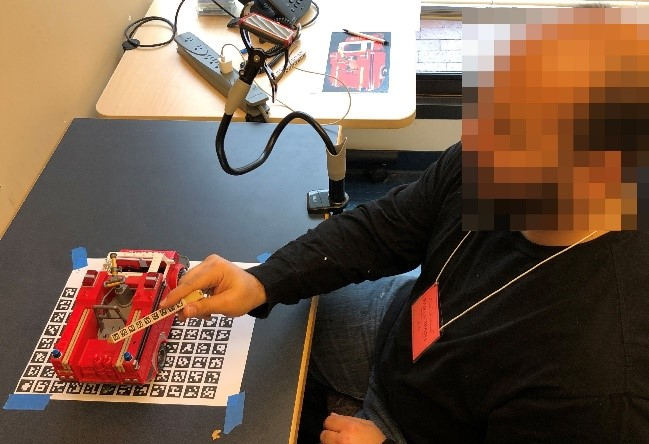
\includegraphics[width=0.58\linewidth,height=4.5cm]{res/img/fig1a}
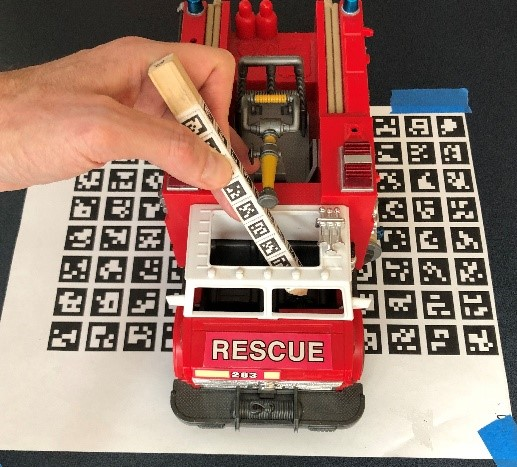
\includegraphics[width=0.42\linewidth,height=4.5cm]{res/img/fig1b} 
%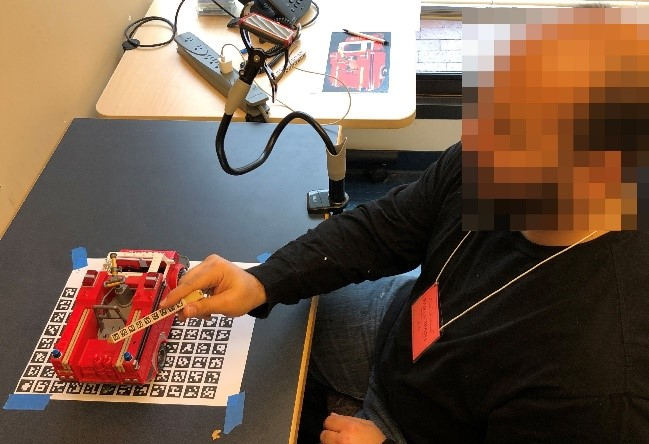
\includegraphics[height=4.5cm\linewidth]{res/img/fig1a}
%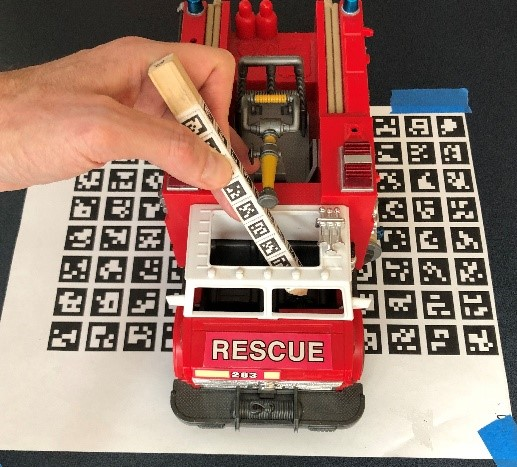
\includegraphics[height=4.5cm\linewidth]{res/img/fig1b} 
\caption{(left) Blind participant uses CamIO to explore a toy fire truck. The participant holds the CamIO {\em stylus} (a barcode pattern printed on a square wooden dowel with a pointy tip) to point to possible hotspots on the truck. The truck is glued to the {\em board} (a piece of paper with a separate barcode pattern), which is taped to the table. An iPhone 8 running CamIO is held by a gooseneck cellphone holder to capture a view of the truck, board and stylus. (right) Stylus points to steering wheel in the truck cabin. Though the steering wheel is in a recessed location that is not visible to CamIO, the stylus tip location can still be estimated.}
\label{fig:exp}
\end{figure}

Each of the 10 hotspots was searched for under both feedback conditions: G (guidance provided) and NG (no guidance). 
In order to minimize the influence of any possible learning effects, which could make it easier to find a hotspot the second time it was searched for, we randomized the sequence of hotspots, and alternated between NG and G trials. With 10 trials in both guidance conditions (G and NG), this resulted in a within-subject factorial design with an identical sequence of $2K = 20$ trials per participant.
The participant was given up to 120 sec. to find each hotspot, after which a time-out was declared.

We had a total of N=4 blind participants in our experiment (2 males/2 females, ages from 26-42).
Participants P1, P3 and P4 were already familiar with the CamIO system (P4 is a co-author of this paper) while P2 was unfamiliar with it. 
None of the participants was told the study design before their trials, and we didn't tell them whether or not any locations would be repeated in the 20 trials. 

After obtaining IRB consent, we reviewed how CamIO works if necessary and demonstrated the audio guidance feature. 
The experimenter launched CamIO on an iPhone 8 and positioned it on a gooseneck cellphone holder so that the camera captured the entire truck and board. 
Each participant spent a short time practicing with the guidance feature (on different hotspots than the one used for the evaluation), with help provided by the experimenter as needed.

In the practice phase, the experimenter explained that barriers sometimes block the user from moving in the suggested guidance direction. 
For instance, if in Fig.~\ref{fig:exp}(right) the system directs the participant to move ``forward'' towards the left side mirror, the stylus will soon hit the cabin roof/wall as it moves towards the mirror; the participant must find ways around such obstacles to find the target hotspot. 

Next each participant performed the formal experimental trials, which consisted of the 20-trial sequence described above. 
We  placed a visual barrier between the participant and the object while the experimenter defined the hotspot in each trial to prevent participants from using any residual vision to see the location of the hotspot. After completing the 20 search trials, we administered a System Usability Scale (SUS) \cite{brooke1996sus} to estimate the usability of the guidance system. 
Finally, we conducted a semi-structured interview asking what participants liked and disliked about the system, what needed to be improved, and how they might envision an ideal guidance system. Since P4 is a co-author on this paper, we did not administer the SUS or semi-structured interview to him.

\hypertarget{results}{%
\section{Results and Discussion}\label{results}}
%%%

Fig.'s~\ref{fig:res-ul}-\ref{fig:res-full} plot the times needed to find the hotspot in both guidance conditions, and Fig.~\ref{fig:res-full} shows the raw times of each participant for each condition and hotspot. All times are in seconds; times reported as 120 secs. correspond to participants failing to find the target in the allotted time.

\begin{figure}
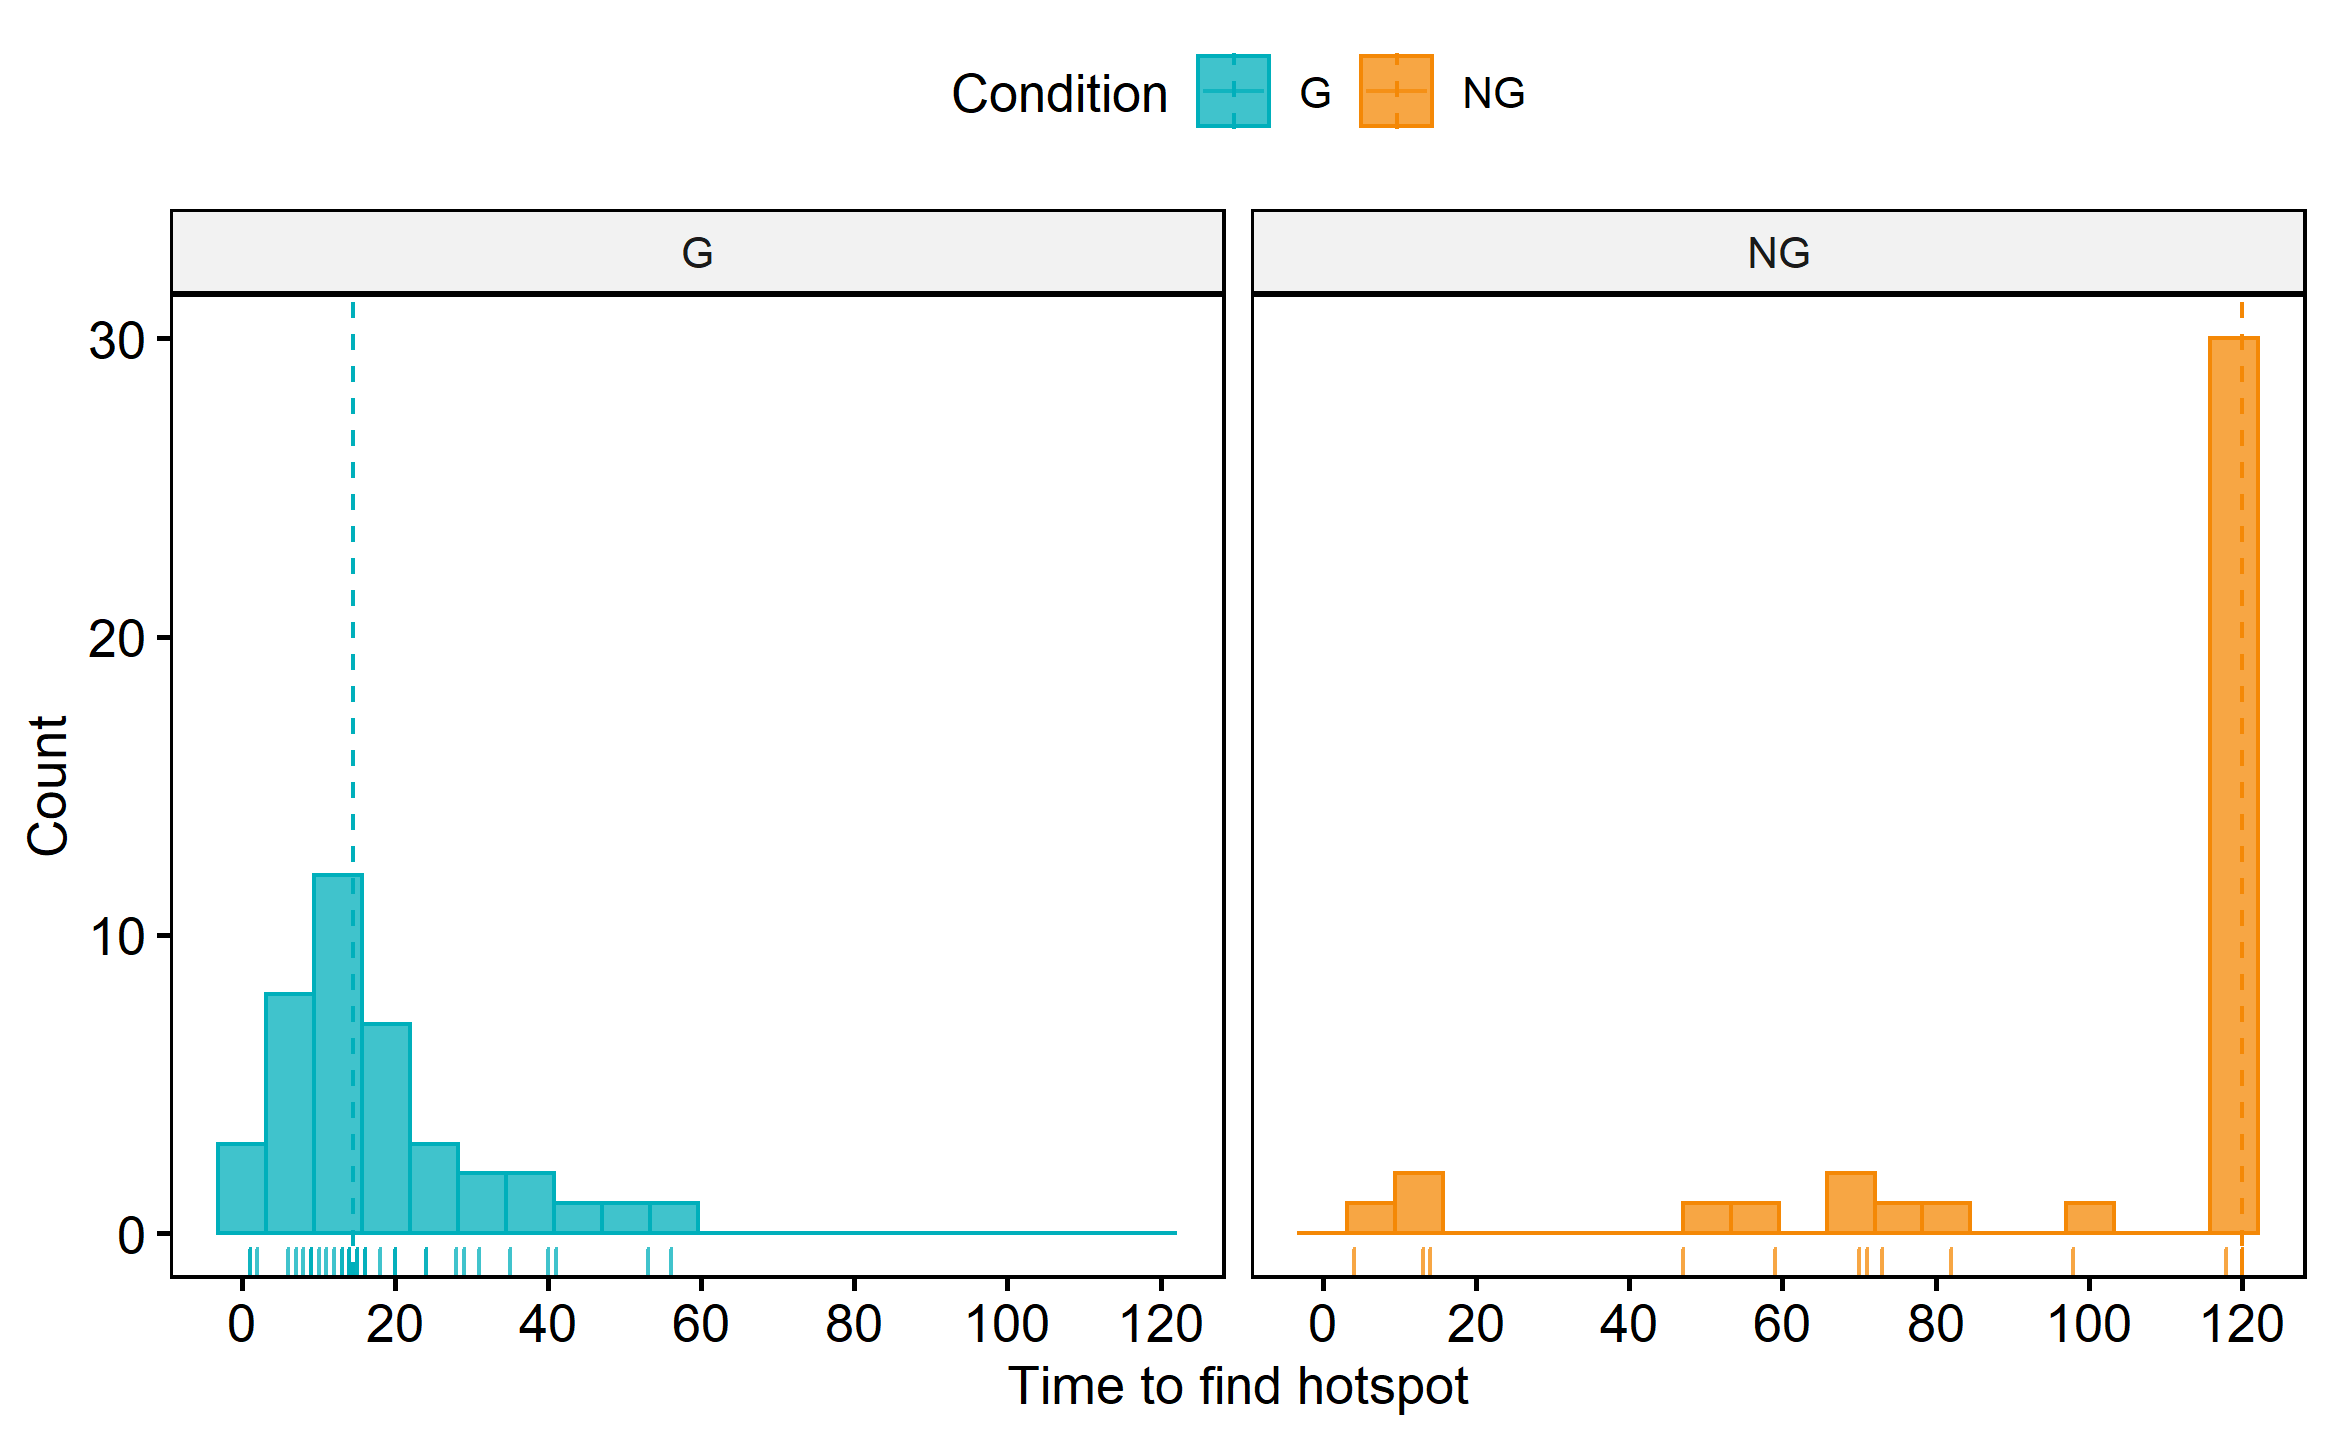
\includegraphics[width=12cm, keepaspectratio,]{res/img/hist.png}
\caption{
Histogram of the times to find the hotspots for each guidance condition, aggregated over participants and hotspots. The vertical dashed lines represent the median scores.}
\label{fig:res-ul}
\end{figure}

\begin{figure}
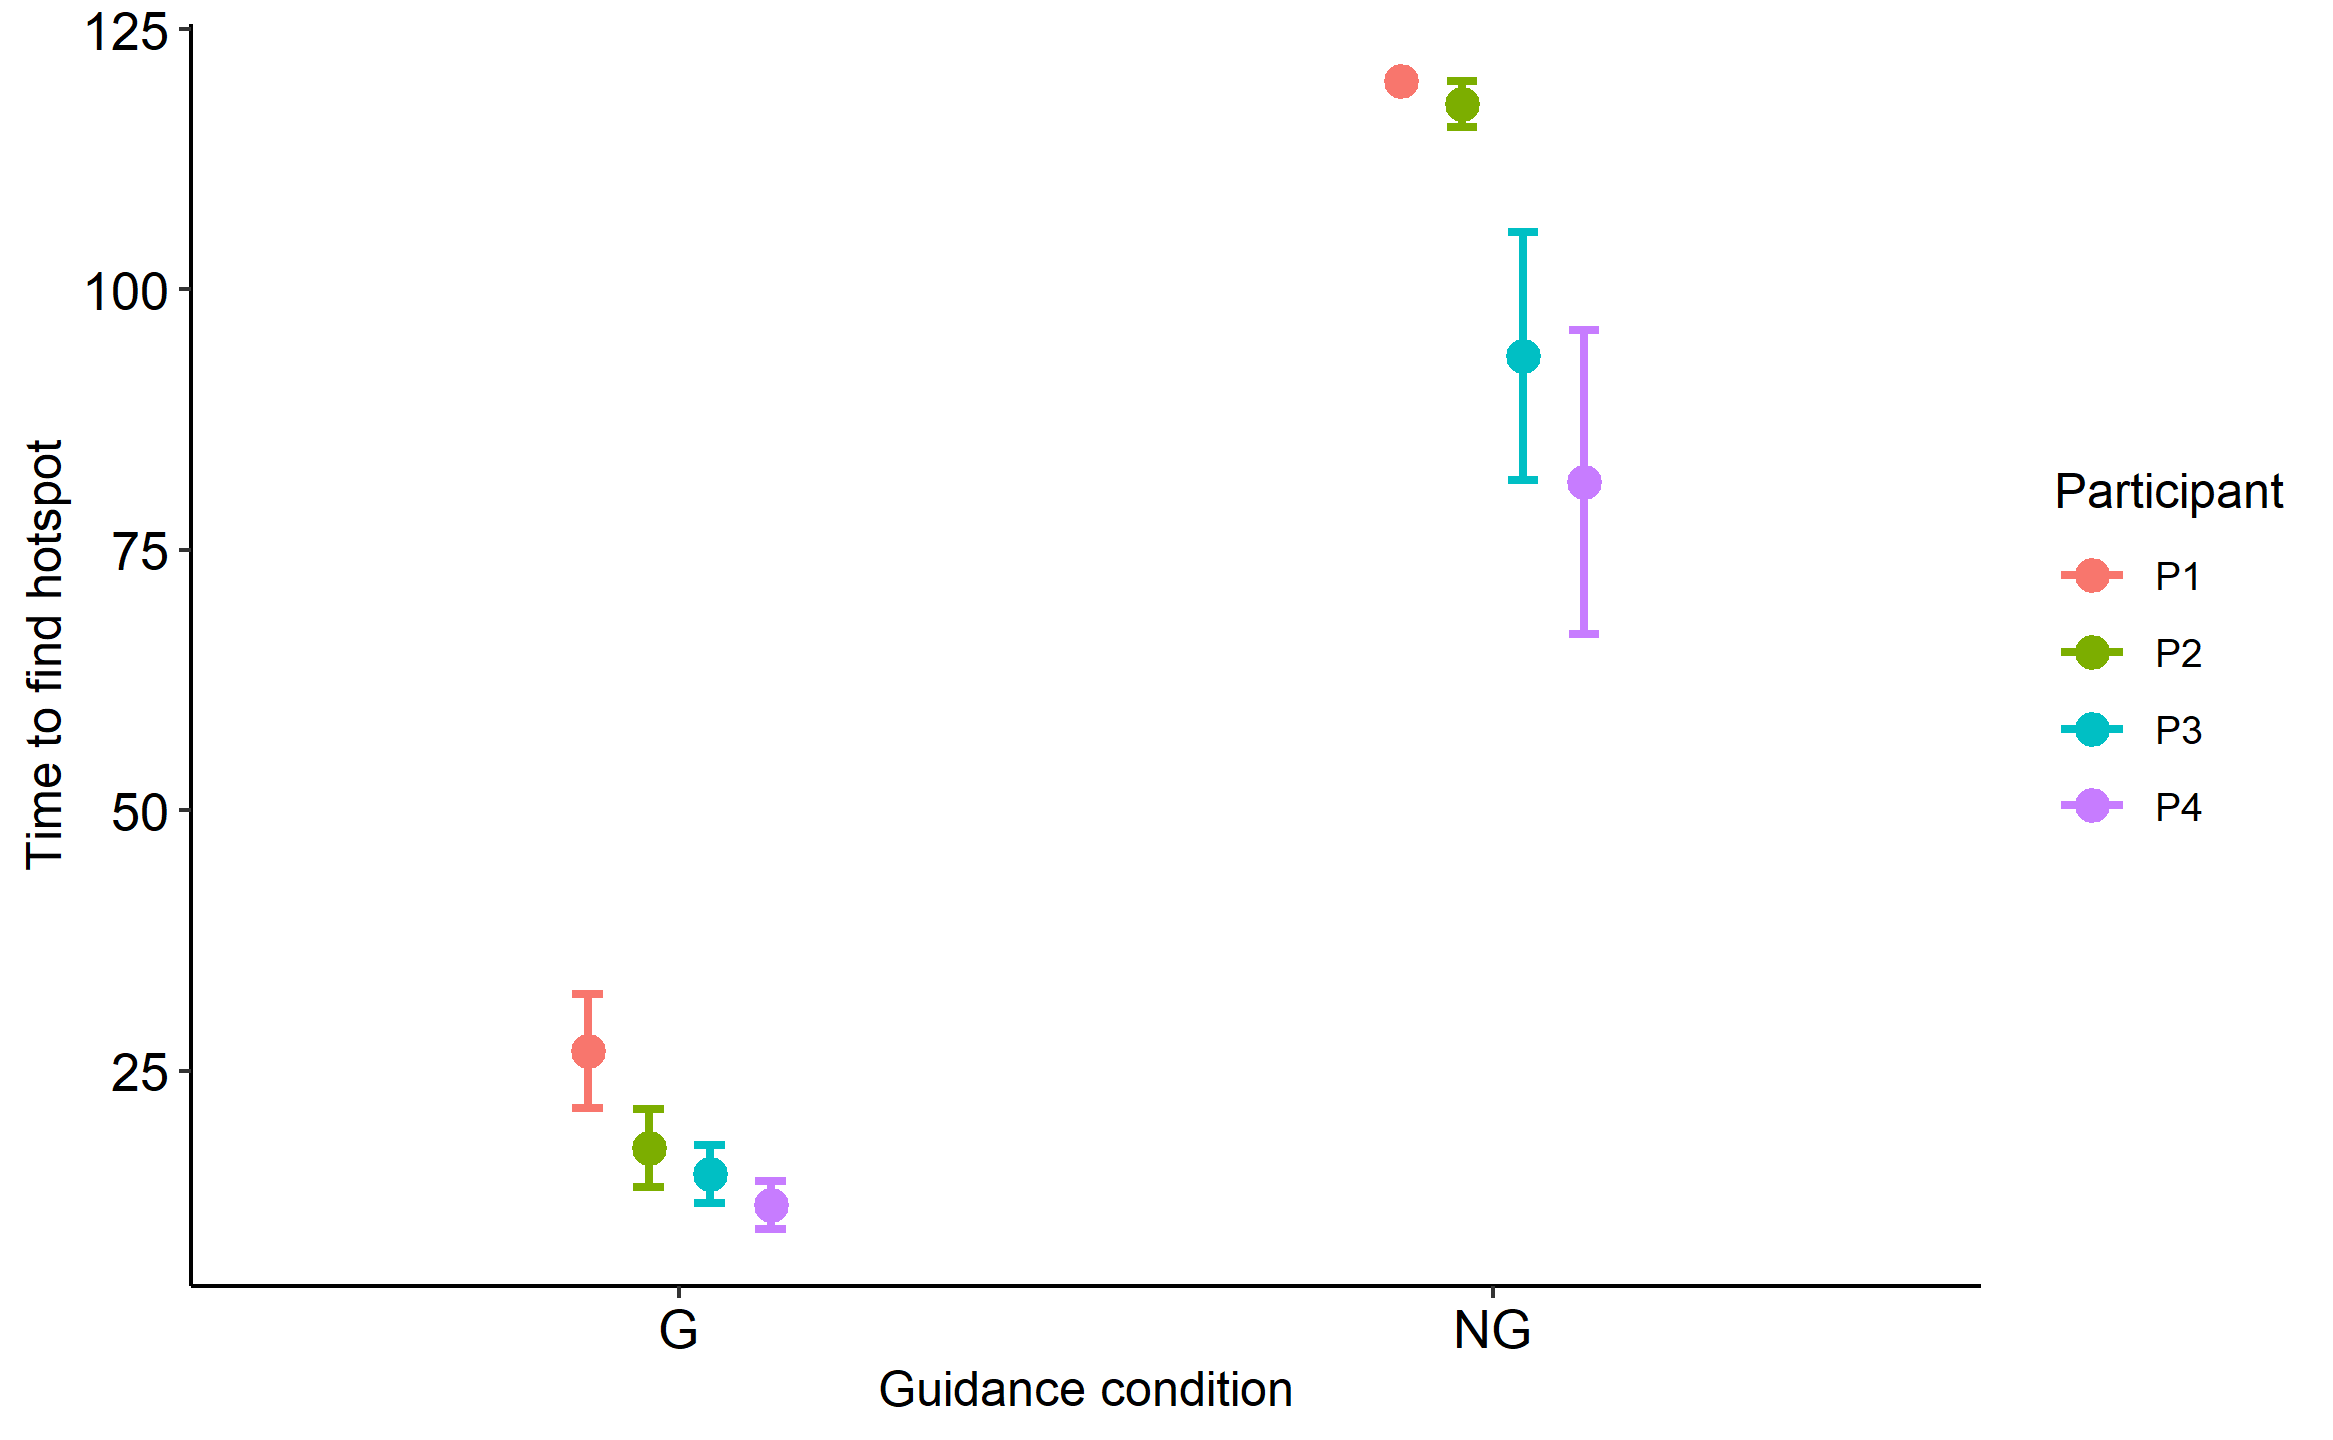
\includegraphics[width=12cm, keepaspectratio,]{res/img/lines.png}
\caption{
Line plot showing the average time to find the hotspot ($\pm{SE}$) per subject and per guidance condition.}
\label{fig:res-ur}
\end{figure}

\begin{figure}
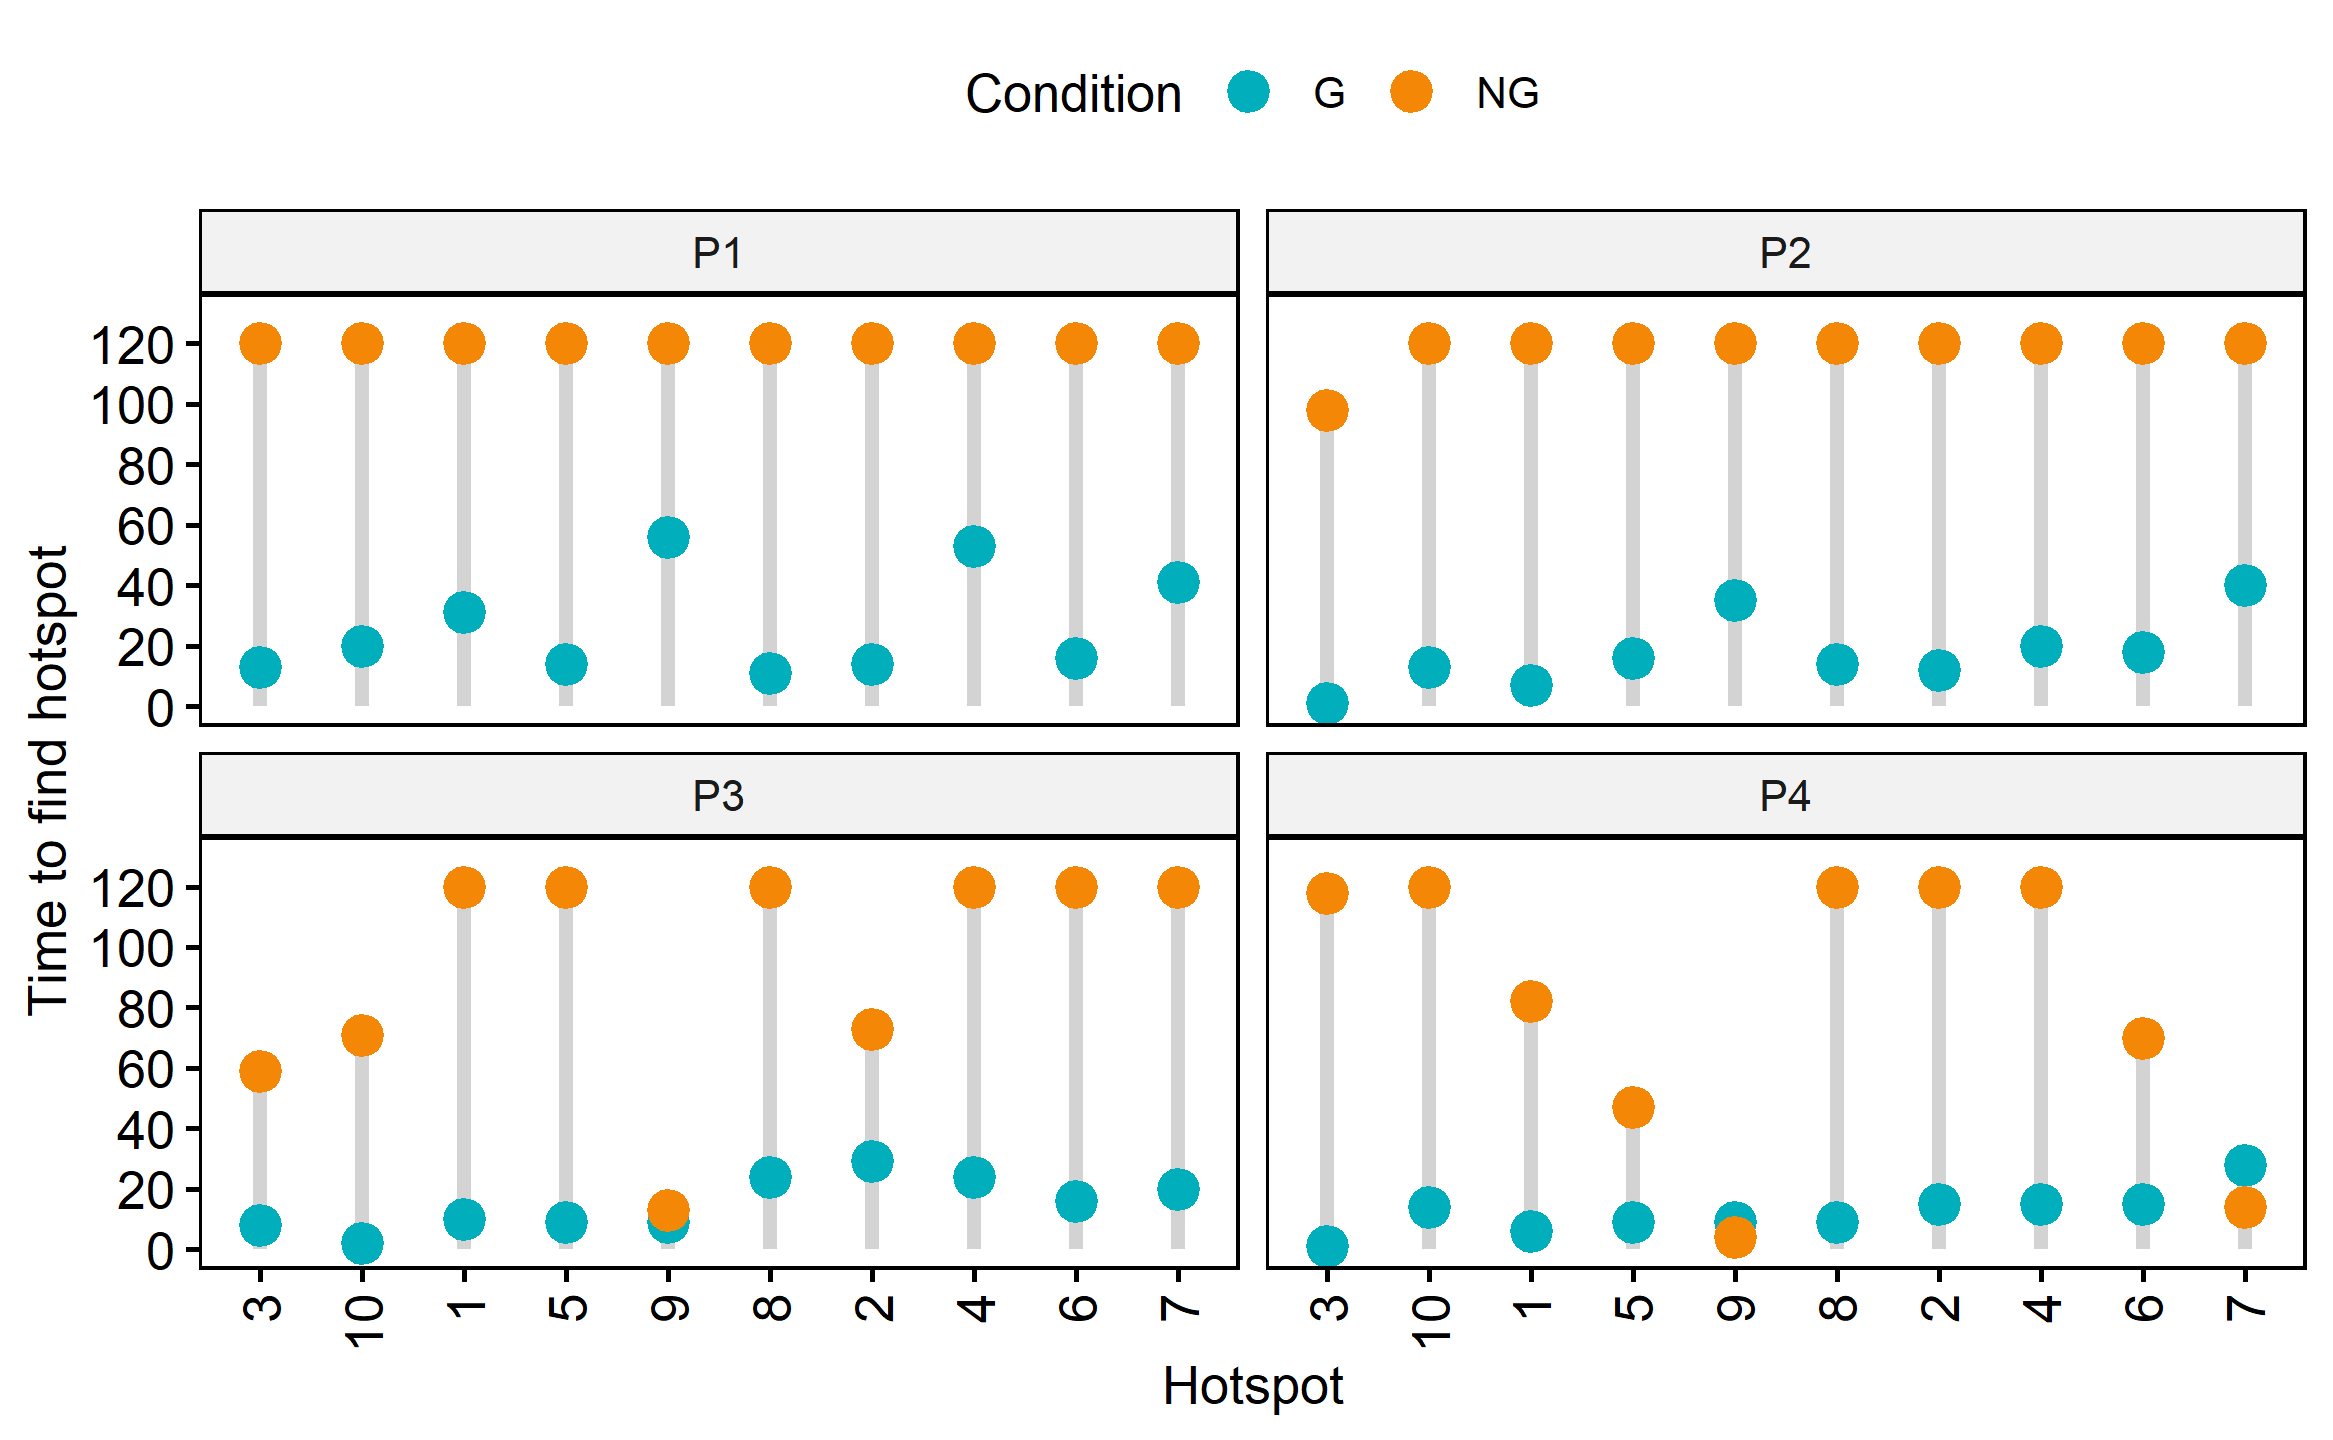
\includegraphics[width=12cm, keepaspectratio,]{res/img/full.png}
\caption{
Time to find target hotspot location for each participant, colored by guidance condition. This plot displays all the raw experimental data.}
\label{fig:res-full}
\end{figure}

These plots show how the time to find the hotspot depends on factors such as the guidance condition (G vs. NG), the participant and which hotspot is the target. Note that G resulted in a successful target search in all cases, and in all but two cases (both for P4), target search took less time with G than with NG (visible in Fig. \ref{fig:res-full}).

We used a Wilcoxon signed-rank test to compare the differences between G and NG times (see Fig.~\ref{fig:res-diff}), paired by hotspot for each participant. The result indicated that participants performed significantly better under condition G (median = 14.5 sec.) than in condition NG (median = 120 sec.), with $V=5$, $Z=5.45$, $p = 5.18 \times 10^{-8}$, and an effect size of $r = 0.86$. 

\begin{figure}[h!]
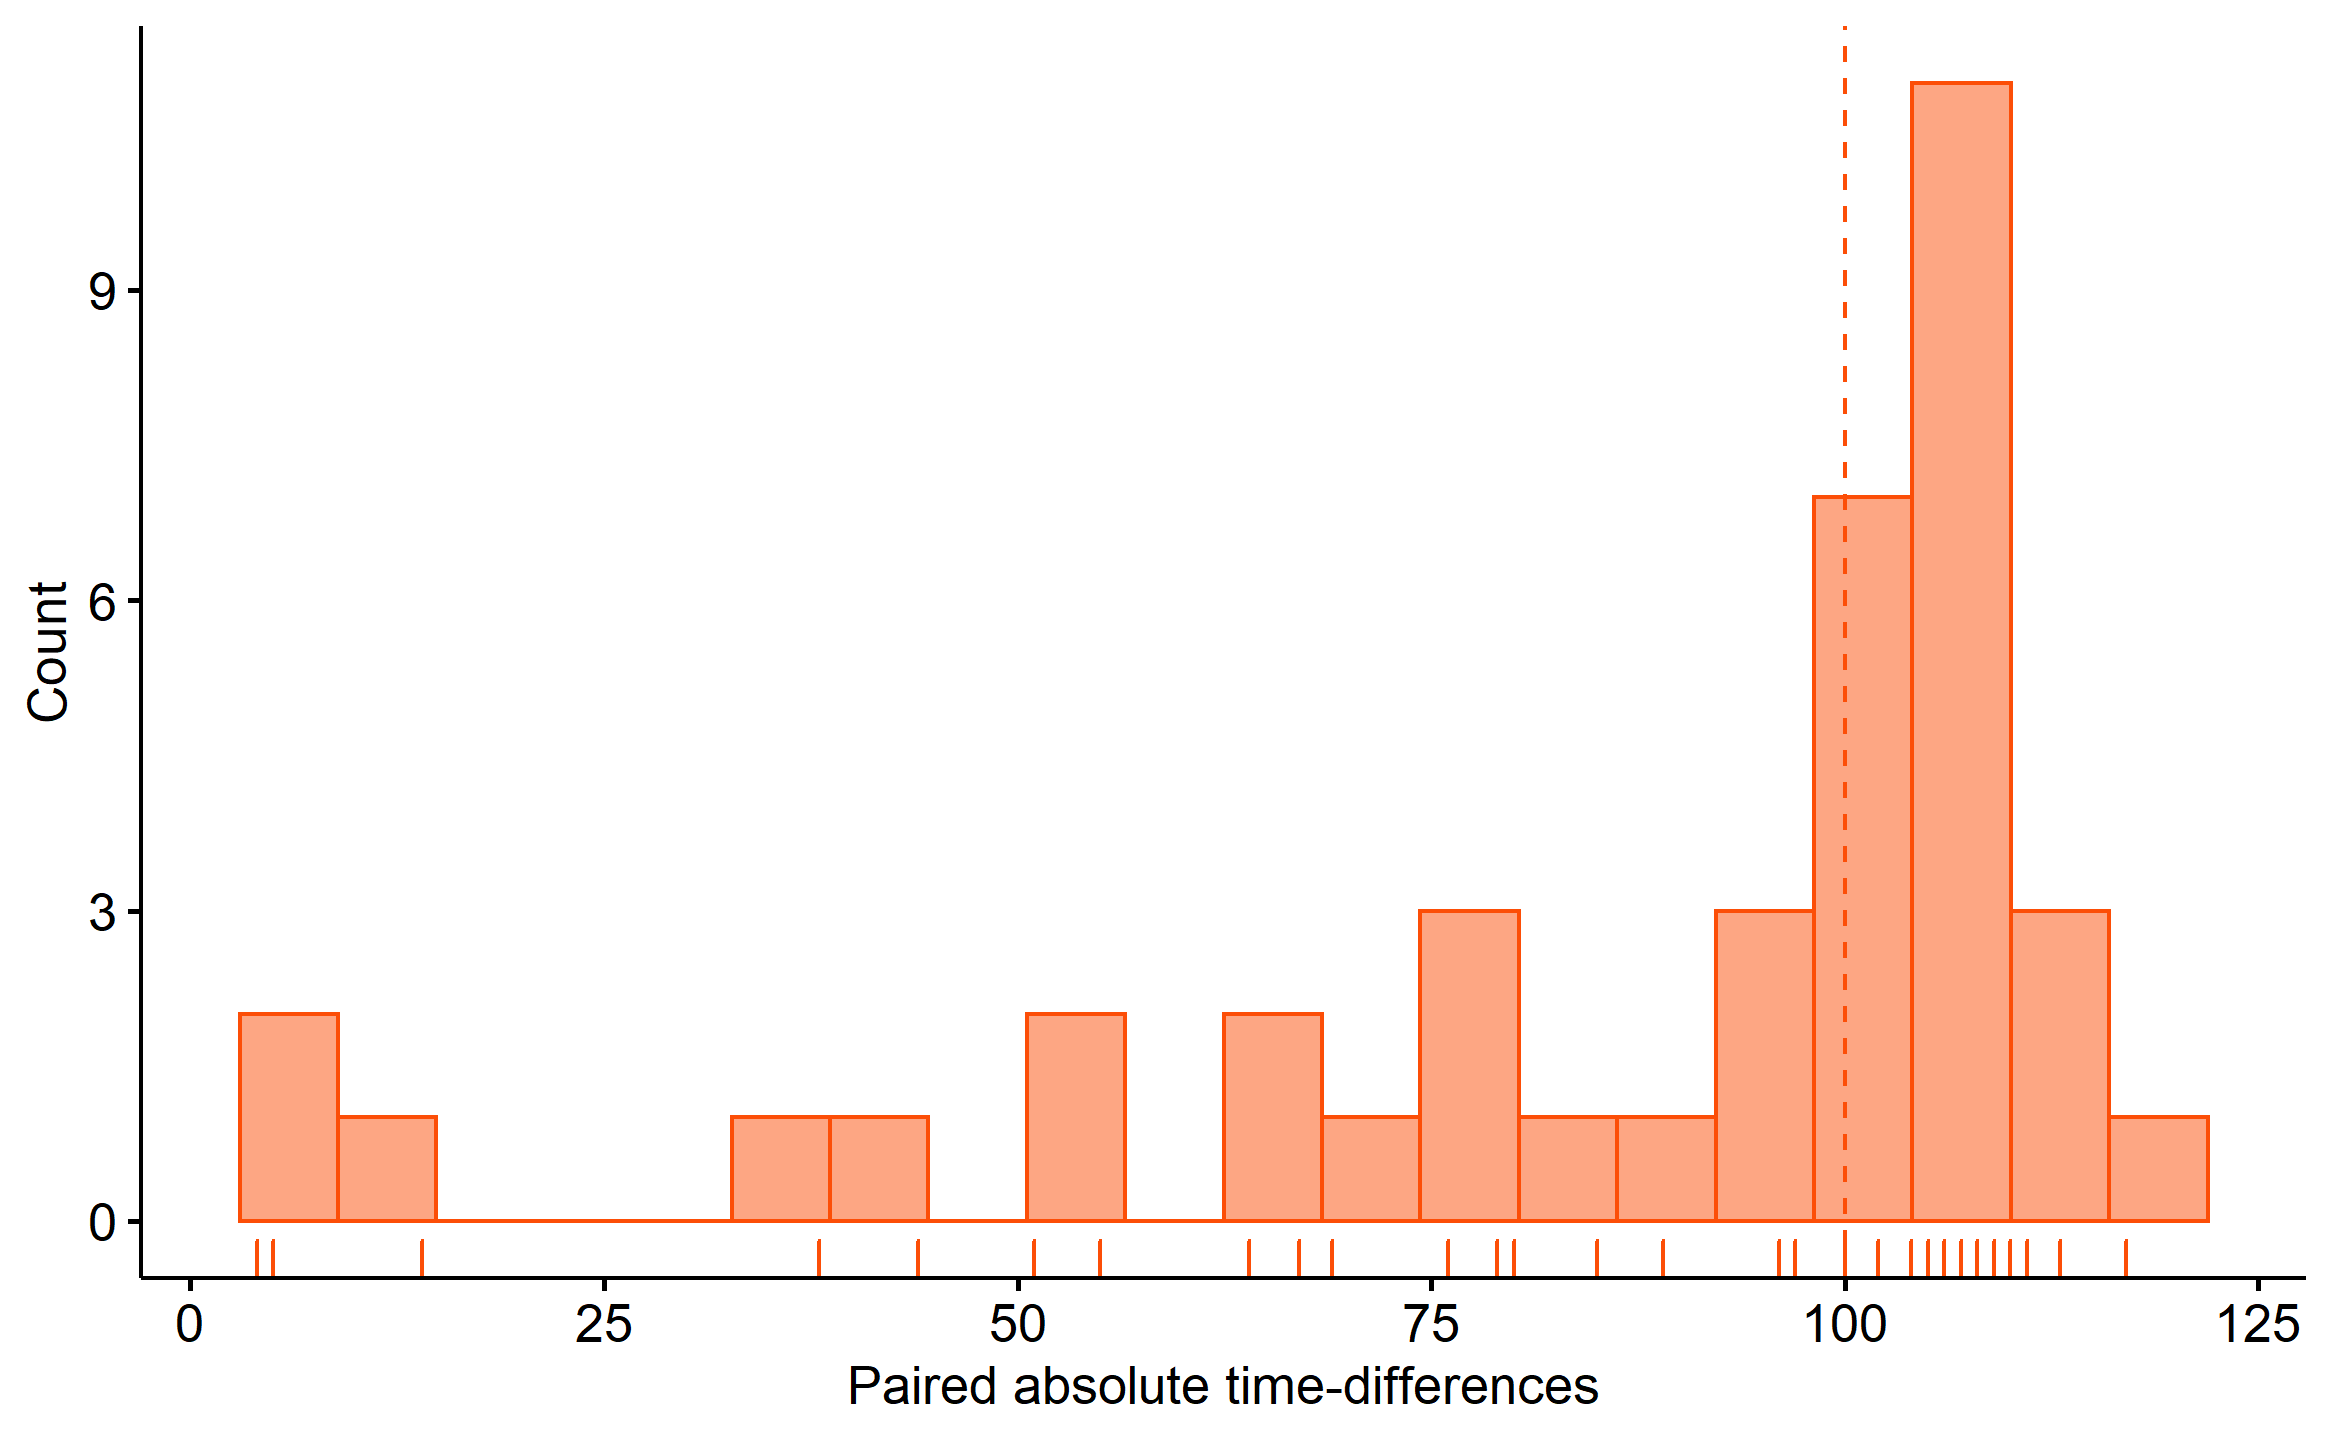
\includegraphics[width=11.5cm, keepaspectratio,]{res/img/hist_diff.png}
\caption{Histogram of the differences (paired by hotspot \& condition) in the time to find hotspots, aggregated over participants. Positive time differences indicate that the time under NG was longer than the time under G.}
\label{fig:res-diff}
\end{figure}

It should be noted that, despite our low number of participants, we had 10 pairs of measurements per participant, and a large effect-size (according to Cohen's guidelines), which should theoretically compensate for the increased type-I error rate risk inherent to running inferential statistics on a small sample.

The following System Usability Scale (SUS) scores were calculated: P1=65, P2=75, P3=77.5, for an average of 72.5. 
An SUS score of 68 is considered ``average'' while scores in the mid- to high 70s are considered ``good''\footnote{\url{https://measuringu.com/interpret-sus-score/}}.
Overall, the SUS scores suggest that the guidance system is usable but needs improvement.

Next we summarize the qualitative feedback we obtained in the semi-structured interviews. 
All participants who provided qualitative feedback (P1, P2 and P3) acknowledged the benefit of the audio guidance that was provided, which they found intuitive and clearly superior to finding hotspots without guidance, or to more indirect ways of providing guidance (such as the early version we implemented that used tempo to signal the distance from the target and pitch to direct the stylus up or down). P3 specifically favored the ``specific'' instructions that the verbal feedback provided to direct the user to a hotspot, which was especially useful when the hotspot was hard to find using tactile cues alone. 

However, P1 and P2 felt that the limited spatial accuracy of the CamIO system was the biggest problem that needed to be addressed; for instance, in some cases the system announced the target had been reached even though the stylus tip was hovering about 1 cm above the truck surface. (This spatial inaccuracy
results from noise in the board pose and stylus tip location estimates.)
P3 expressed frustration with time lag, i.e., the voice feedback tended to lag behind the current location of the stylus, even when she was moving the stylus slowly; she also felt that the speed of the repetitive speech feedback made her feel rushed.

When asked what improvements the participants wanted, P1 suggested equipping the stylus with a button that turns on the guidance feedback, and the addition of multiple vibrators on the stylus that could provide haptic feedback indicating which way the stylus should be moved. 
P2 suggested adding audio information similar to the earlier guidance system that the authors experimented with (Sec. 3), which would use a combination of tempo, pitch and volume changes to signal when the stylus gets closer to the target location. 
P3 expressed the desire that CamIO work with any ordinary pen or pencil, rather than requiring the special stylus we used.

\hypertarget{conclusion}{%
\section{Conclusion}\label{conclusion}}

We have devised a 3D spatial guidance system that helps a blind user find a specific location of interest on an object using CamIO, an audio-based AR system. 
The guidance system uses simple verbal commands (``left'', ``right'', ``up'', etc.) to tell the user which direction to
move the stylus tip. Experiments with four blind participants show that the guidance system significantly speeds up the search for target hotspots compared with an exhaustive search. 
A secondary contribution of this study is to demonstrate the ability of the CamIO stylus to access recessed or otherwise obscured locations on an object that are not themselves visible to the camera.

While we applied this guidance approach specifically to CamIO, it could be useful in any AR system, whether the system tracks the user's hands, handheld stylus or other pointing tool. 
Such audio-based guidance is not only helpful for blind users but is also useful in applications where visibility is limited (either by environmental conditions or because of a visual impairment), or for sighted users who prefer a cross-sensory display (e.g., audio and visual combined).

Future work will focus on refining and improving the audio interface.
One possible way to speed up the guidance process is to add more specific directional feedback, e.g., ``far left'' would tell the user to move the stylus farther to the left than the ``left'' instruction. 
The verbal directions could be augmented with 3D spatialized sound as in \cite{mayAuditoryDisplaysFacilitate2019}, which could make the guidance more intuitive. 
Finally, we will continue to test and improve the CamIO system, with an emphasis on refining the spatial accuracy of the tip location estimates using improved computer vision algorithms.

\section{Acknowledgments}
JMC, BB and HS were supported by NIH grant 5R01EY025332 and NIDILRR grant 90RE5024-01-00. We thank Dr. Roberto Manduchi, Dr. Natela Shanidze, Dr. Santani Teng and Dr. Ali Cheraghi for helpful suggestions about the experiments.


% ---- Bibliography ----
\bibliographystyle{res/templates/splncs04}
\bibliography{res/refs.bib}

\end{document}